\section{Characterization of MAPMTs}
The performance of MAPMTs was evaluated under certain high voltages.
The single photoelectron spectrum and the pixel efficiency for H12700 MA-PMTs were tested and analyzed at 1000v, 1050v, 1075v, and 1100v.
The measurements performed at the reference supply voltage of 1000 V were compared to the measurements at different HV values in order to study the behavior of the MAPMT response as a function of the supply voltage.
As expected, it was found that the H12700 MA-PMTs perform the best in the single photoelectron spectrum efficiency at higher voltages, especially at 1100v.
We see a significantly improved separation of the first photoelectron peak from the pedestal at higher voltage supplies (see~Fig.~\ref{fig:SPEhv}).
When the average deficiencies of the tested MA-PMTs were analyzed, it was found that the average efficiency for 1000v, 1050v, 1075v and 1100v were approximately 4.6\%, 4.9\%, 5.0\%, and 5.2\%, respectively.
Therefore, the increase in detection efficiency is found to be over 10\% at 1100 V in comparison to 1000 V supply.
This separation is the crucial point for a single photon counting detectors such as CLAS12 RICH, where the occupancy is at the level of one photon per pixel.

\begin{figure}[b]
	\centering
	\centering
	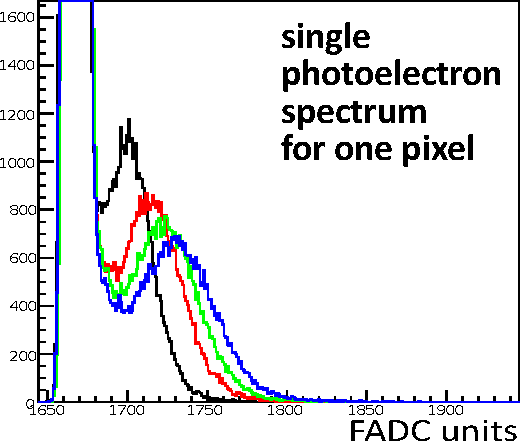
\includegraphics[width=0.8\linewidth]{SPEhv.pdf}
	\captionof{figure}{SPE spectra at 1000 (black), 1050 (red), 1075 (green) and 1100 (blue) V.}
	\label{fig:SPEhv}
\end{figure}



It was also found that as the gain of the MAPMT increased, the efficiency ratio of 1100v to 1000v decreased.
The ratio is shown on~Fig.~\ref{fig:effratio} as a function of MAPMT gain reported by Hamamatsu.
The high voltage supply improves the performance of MAPMT dynode system, decreasing the fraction of the single photoelectron events below the pedestal peak.
This indicates that lower gain MAPMTs have a greater difference in the efficiencies at 1100v and 1000v, while higher gain MAPMTs have a smaller difference between the two voltage efficiencies.
The improvement for lower gain MAPMTs is more significant than for higher gain MAPMTs, because the high gain MAPMT has good separation of signal from pedestal even at the reference 1000 V.
Therefore, the low gain MAPMT benefit greatly from higher supply voltage.
The collected data are used to determine what high voltage the MAPMTs should be ran at to acquire the best results when the RICH detector is completed.


\begin{figure}[bt]
	\centering
	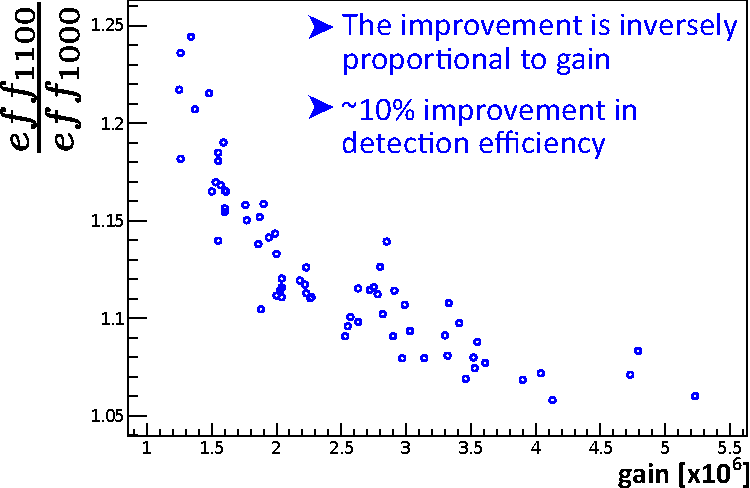
\includegraphics[width=0.8\linewidth]{effratio.pdf}
	\caption{Ratio of MAPMT efficiencies at 1100 and 1000 V as a function of MAPMT gain.}
	\label{fig:effratio}
\end{figure}

The parameters from Pavel's PMT response function are shown on the Fig.~\ref{fig:mu} and \ref{fig:characteristicPars} and correspond to the emission of the photoelectron ($\mu$), its collection and multiplication on the first dynode ($scale$ and $\nu$).
We have omitted other parameters that take into account the resolution effects of readout system or correspond to the cascade multiplication of the secondary electrons as they are out of scope focus of our analysis.
Given our requirements for single photoelectron signal sensitivity MAPMTs of our choice should be able to detect with high probablity single photon that reaches photocathode.
In order to achieve this goal MAPMT should have high quantum efficiency of the photocathode as well as high collection efficiency of produced photoelectron combined with substantial signal multiplication to achieve good resolution of SPE peak.
These characteristics were studied in bulk for all 27520 channels (430x64) during the different light conditions and for different supplied HV values.

\begin{figure}[bt]
	\centering
	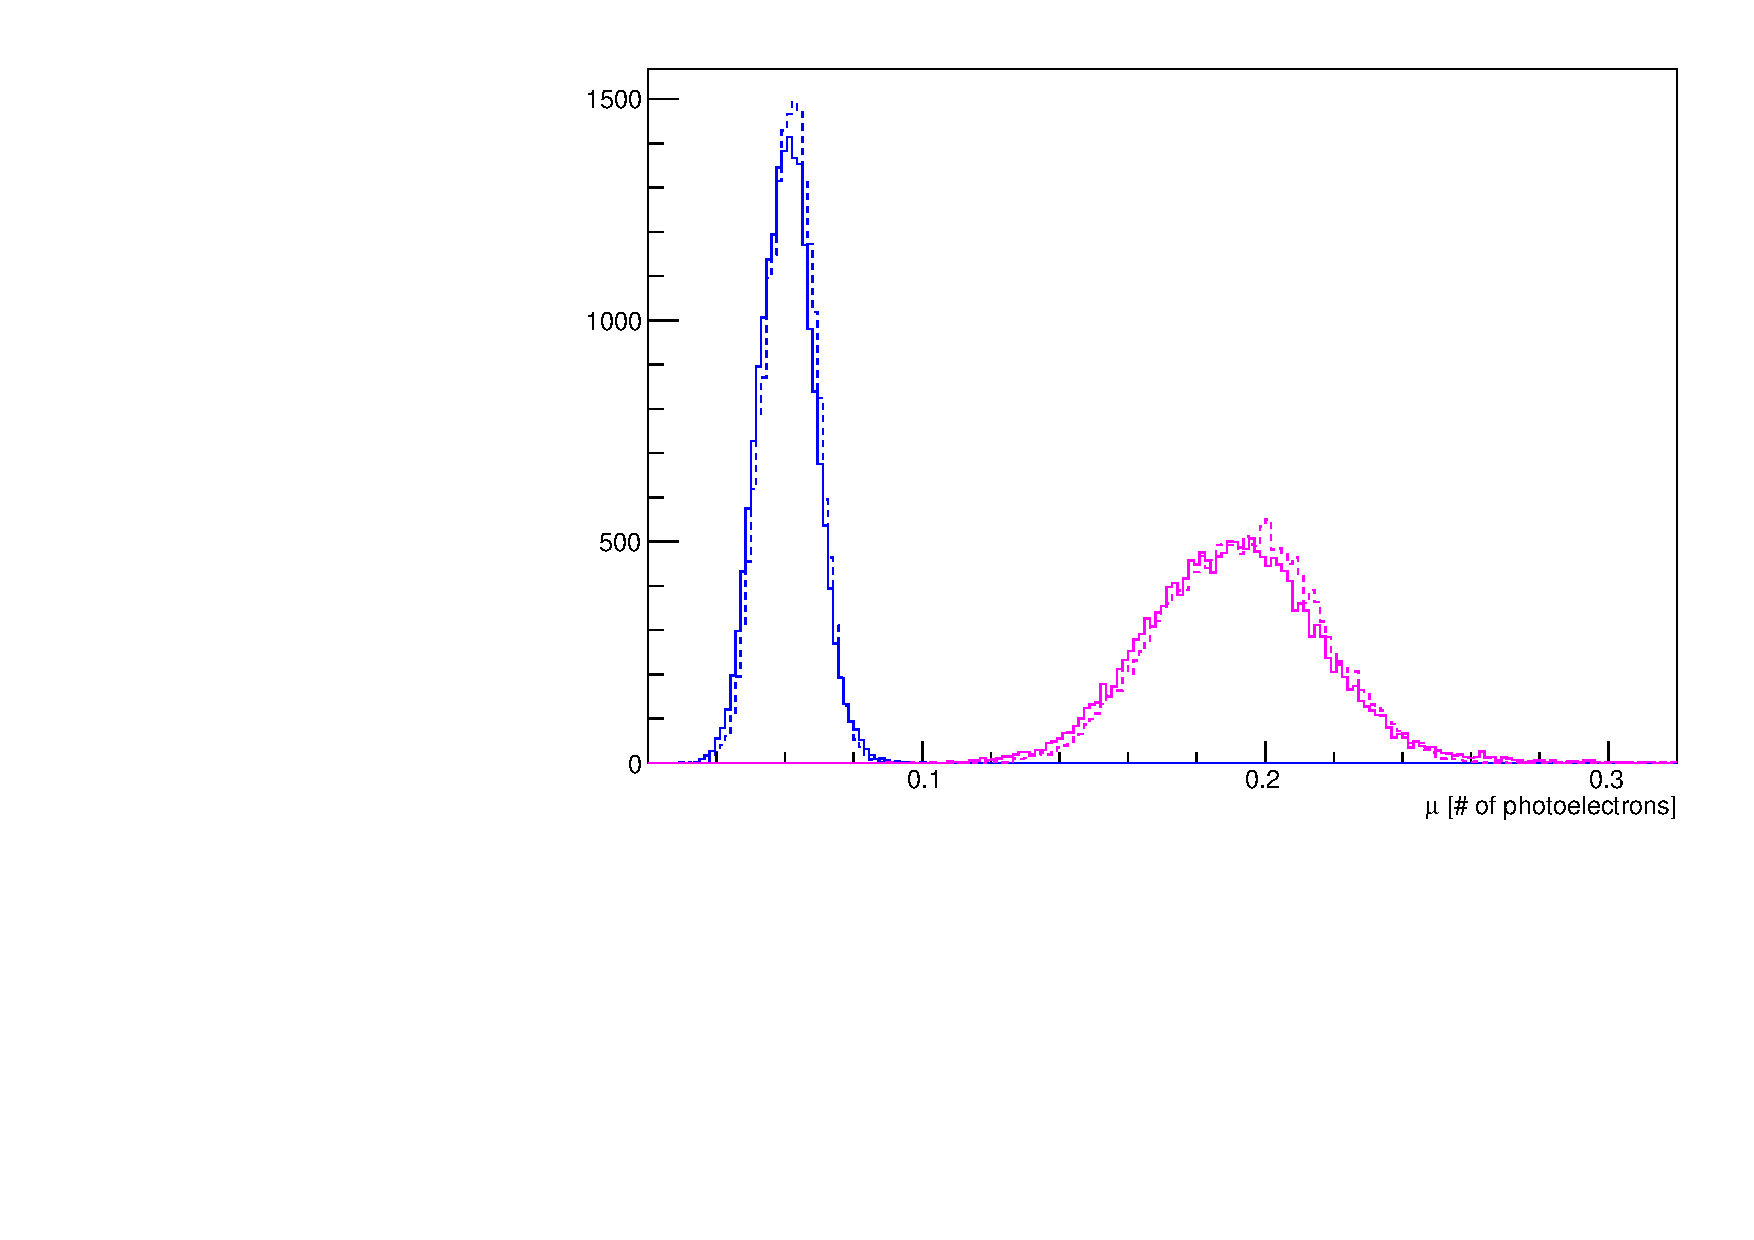
\includegraphics[width=0.8\linewidth]{mu.pdf}
	\caption{Average number of the photoelectrons emitted from the photocathode for different laser light intensities: $10^{-5.4}$ - blue and $10^{-4.6}$ - red. Solid line is for measurements at 1000 V and dashed - at 1100 V}
	\label{fig:mu}
\end{figure}

Fig.~\ref{fig:mu} shows the distribution of parameter $\mu$ which correspond to the average number of the photoelectrons produced during the measurements.
This parameters represents the convolution of the MAPMT photocathode quantum efficiency and laser setup light intensity.
Both characteristics should not depend on HV supply values and it is demonstrated on this figure by comparison of $\mu$ values extracted for the measurements at 1000 V and 1100 V.
However one can change the parameter by varying the laser light intensity which is evident from the left shift of $\mu$ values for lower light intensity measurements.

The other two free parameters are plotted on Fig.~\ref{fig:characteristicPars}.
They correspond to the average number of second-stage electrons produced on the first dynode by photoelectron (see~Fig.~\ref{fig:nu} and average signal amplitude for single photoelectron spectrum (see Fig.~{fig:scale}).
Both parameters characterize mainly the amplifying subsystem of MAPMT and therefore should depend on supplied HV.
The measurements at 1000 V and 1100 V confirm that amplification is improved at higher values of applied high voltage.
Traditionally the second parameter (gain) is often used to describe the amplification abilities of photomultipliers and often used in calibration and reconstruction procedures.
And it was shown that the extracted gains do not depend on the light conditions with a high degree of accuracy.

\begin{figure}[b]
	\centering
	\begin{subfigure}{0.48\linewidth}
	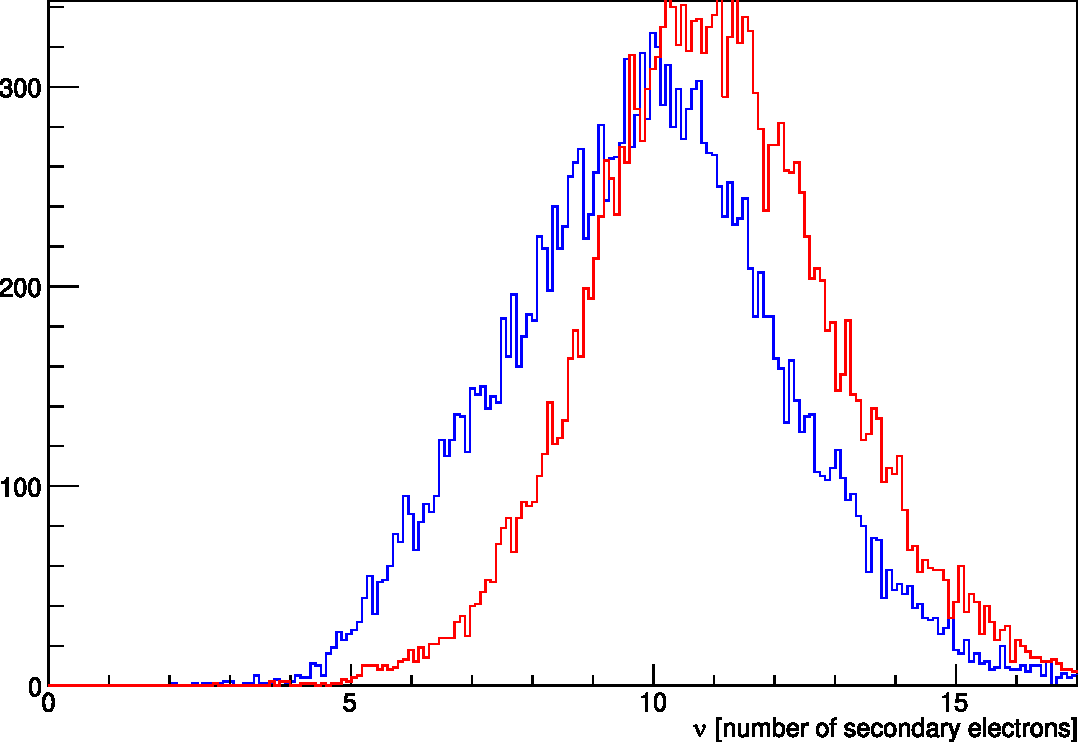
\includegraphics[width=\linewidth]{nu.pdf}
	\caption{}
	\label{fig:nu}

	\end{subfigure}
	\begin{subfigure}{0.48\linewidth}
	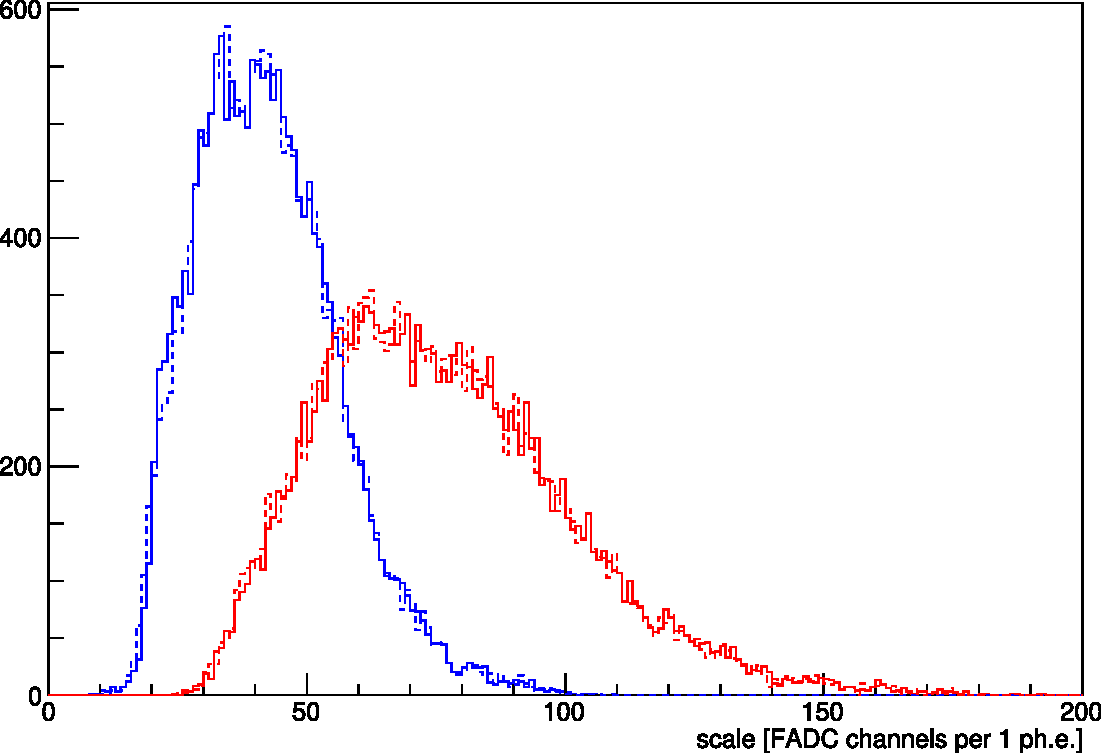
\includegraphics[width=\linewidth]{scale.pdf}
	\caption{}
	\label{fig:scale}
	\end{subfigure}

	\caption{Characteristic parameters of single photoelectron signal distributions from Hamamatsu H12700 MAPMT in the framework of Pavel Degtiarenko's model for measurements at different HV: 1000 V (blue) and 1100 V (red):
		(a) average number of second-stage electrons knocked out of the first dynode,
		(b) the average signal amplitude per single photoelectron for different light intensity measurements: at $10^{-5.4}$ (solid line) and at $10^{-4.6}$ (dashed) attenuation}
	\label{fig:characteristicPars}
\end{figure}


